\chapter{Deuteronomy 15}

\begin{figure}
  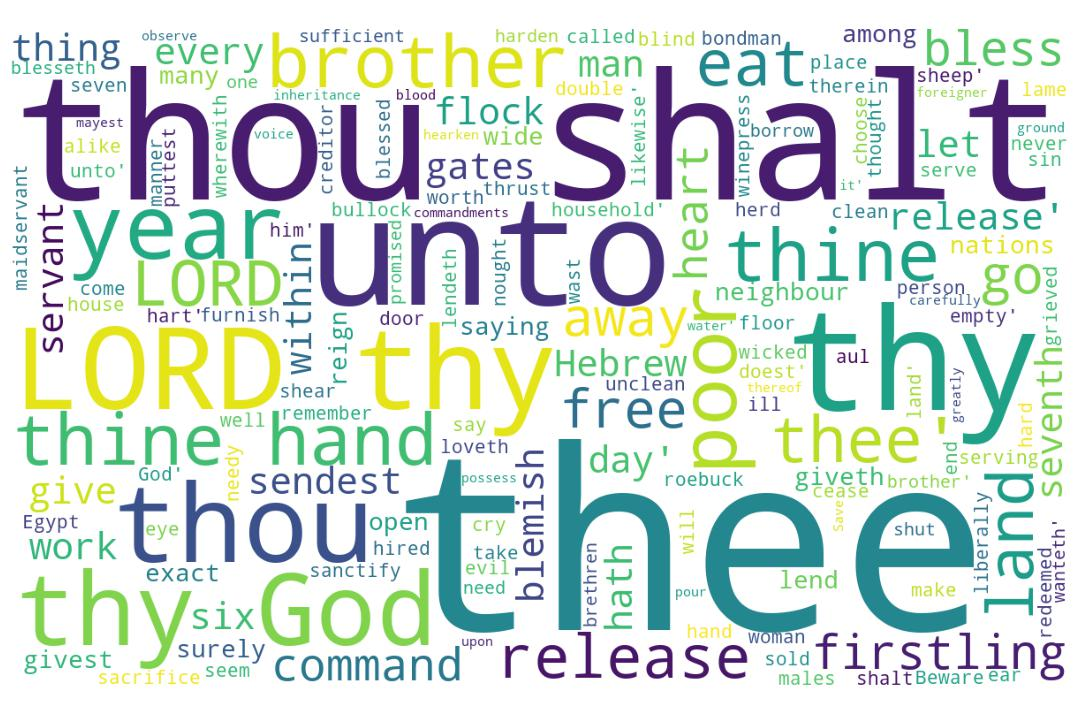
\includegraphics[width=\linewidth]{05OT-Deuteronomy/Deuteronomy15-WordCloud.jpg}
  \caption{Deuteronomy 15 Word Cloud}
  \label{fig:Deuteronomy 15 word Cloud}
\end{figure}

\marginpar{\scriptsize \centering \fcolorbox{bone}{lime}{\textbf{PRINCIPLES OF THE SABBATH}}\\ (Deuteronomy 15:1-23) \begin{compactenum}[I.][8]
    \item  The \textbf{Sabbath}  %\index[scripture]{Deuteronomy!Deu 15:09} \index[scripture]{Deuteronomy!Deu 15:11} (Deuteronomy 19:9, 11)
    \item  \textbf{Sufficiency}  \index[scripture]{Deuteronomy!Deu 15:08} (Deu 15:8)
    \item  The \textbf{Sayings of God}  \index[scripture]{Deuteronomy!Deu 15:09} \index[scripture]{Deuteronomy!Deu 15:11} (Deu 15:9, 11)
    \item  The \textbf{Seventh Year}  \index[scripture]{Deuteronomy!Deu 15:09} \index[scripture]{Deuteronomy!Deu 15:12} (Deu 15:9, 12)
    \item  The \textbf{Sending}  \index[scripture]{Deuteronomy!Deu 15:13}  (Deu 15:13)
    \item  The \textbf{Servants}  \index[scripture]{Deuteronomy!Deu 15:17} \index[scripture]{Deuteronomy!Deu 15:17} (Deu 15:17, 18)
    \item  \textbf{Society}  %\index[scripture]{Deuteronomy!Deu 15:09} \index[scripture]{Deuteronomy!Deu 15:11} (Deuteronomy 19:9, 11)
    \item  Something to \textbf{Sanctify}  \index[scripture]{Deuteronomy!Deu 15:19} (Deu 15:19)
\end{compactenum}}



\footnote{\textcolor[cmyk]{0.99998,1,0,0}{\hyperlink{TOC}{Return to end of Table of Contents.}}}\footnote{\href{https://audiobible.com/bible/deuteronomy_15.html}{\textcolor[cmyk]{0.99998,1,0,0}{Deuteronomy 15 Audio}}}\textcolor[cmyk]{0.99998,1,0,0}{At the end of \emph{every} seven years thou shalt make a release.}
[2] \textcolor[cmyk]{0.99998,1,0,0}{And this \emph{is} the manner of the release: Every creditor that lendeth \emph{ought} unto his neighbour shall release \emph{it}; he shall not exact \emph{it} of his neighbour, or of his brother; because it is called the LORD'S release.}
[3] \textcolor[cmyk]{0.99998,1,0,0}{Of a foreigner thou mayest exact \emph{it} \emph{again}: but \emph{that} which is thine with thy brother thine hand shall release;}
[4] \textcolor[cmyk]{0.99998,1,0,0}{Save when there shall be no poor among you; for the LORD shall greatly bless thee in the land which the LORD thy God giveth thee \emph{for} an inheritance to possess it:}
[5] \textcolor[cmyk]{0.99998,1,0,0}{Only if thou carefully hearken unto the voice of the LORD thy God, to observe to do all these commandments which I command thee this day.}
[6] \textcolor[cmyk]{0.99998,1,0,0}{For the LORD thy God blesseth thee, as he promised thee: and thou shalt lend unto many nations, but thou shalt not borrow; and thou shalt reign over many nations, but they shall not reign over thee.}\\
\\
\P \textcolor[cmyk]{0.99998,1,0,0}{If there be among you a poor man of one of thy brethren within any of thy gates in thy land which the LORD thy God giveth thee, thou shalt not harden thine heart, nor shut thine hand from thy poor brother:}
[8] \textcolor[cmyk]{0.99998,1,0,0}{But thou shalt open thine hand wide unto him, and shalt surely lend him \fcolorbox{bone}{lime}{sufficient} for his need, \emph{in} \emph{that} which he wanteth.}
[9] \textcolor[cmyk]{0.99998,1,0,0}{Beware that there be not a thought in thy wicked heart, \fcolorbox{bone}{lime}{saying}, The \fcolorbox{bone}{lime}{seventh} year, the year of release, is at hand; and thine eye be evil against thy poor brother, and thou givest him nought; and he cry unto the LORD against thee, and it be sin unto thee.}
[10] \textcolor[cmyk]{0.99998,1,0,0}{Thou shalt surely give him, and thine heart shall not be grieved when thou givest unto him: because that for this thing the LORD thy God shall bless thee in all thy works, and in all that thou puttest thine hand unto.}
[11] \textcolor[cmyk]{0.99998,1,0,0}{For the poor shall never cease out of the land: therefore I command thee, \fcolorbox{bone}{lime}{saying}, Thou shalt open thine hand wide unto thy brother, to thy poor, and to thy needy, in thy land.}\\
\\
\P \textcolor[cmyk]{0.99998,1,0,0}{\emph{And} if thy brother, an Hebrew man, or an Hebrew woman, be sold unto thee, and serve thee six years; then in the \fcolorbox{bone}{lime}{seventh} year thou shalt let him go free from thee.}
[13] \textcolor[cmyk]{0.99998,1,0,0}{And when thou sendest him out free from thee, thou shalt not let him go away empty:}
[14] \textcolor[cmyk]{0.99998,1,0,0}{Thou shalt furnish him liberally out of thy flock, and out of thy floor, and out of thy winepress: \emph{of} \emph{that} wherewith the LORD thy God hath blessed thee thou shalt give unto him.}
[15] \textcolor[cmyk]{0.99998,1,0,0}{And thou shalt remember that thou wast a bondman in the land of Egypt, and the LORD thy God redeemed thee: therefore I command thee this thing to day.}
[16] \textcolor[cmyk]{0.99998,1,0,0}{And it shall be, if he say unto thee, I will not go away from thee; because he loveth thee and thine house, because he is well with thee;}
[17] \textcolor[cmyk]{0.99998,1,0,0}{Then thou shalt take an aul, and thrust \emph{it} through his ear unto the door, and he shall be thy \fcolorbox{bone}{lime}{servant} for ever. And also unto thy maidservant thou shalt do likewise.}
[18] \textcolor[cmyk]{0.99998,1,0,0}{It shall not seem hard unto thee, when thou sendest him away free from thee; for he hath been worth a double hired \fcolorbox{bone}{lime}{servant} \emph{to} \emph{thee}, in serving thee six years: and the LORD thy God shall bless thee in all that thou doest.}\\
\\
\P \textcolor[cmyk]{0.99998,1,0,0}{All the firstling males that come of thy herd and of thy flock thou shalt \fcolorbox{bone}{lime}{sanctify} unto the LORD thy God: thou shalt do no work with the firstling of thy bullock, nor shear the firstling of thy sheep.}
[20] \textcolor[cmyk]{0.99998,1,0,0}{Thou shalt eat \emph{it} before the LORD thy God year by year in the place which the LORD shall choose, thou and thy household.}
[21] \textcolor[cmyk]{0.99998,1,0,0}{And if there be \emph{any} blemish therein, \emph{as} \emph{if} \emph{it} \emph{be} lame, or blind, \emph{or} \emph{have} any ill blemish, thou shalt not sacrifice it unto the LORD thy God.}
[22] \textcolor[cmyk]{0.99998,1,0,0}{Thou shalt eat it within thy gates: the unclean and the clean \emph{person} \emph{shall} \emph{eat} \emph{it} alike, as the roebuck, and as the hart.}
[23] \textcolor[cmyk]{0.99998,1,0,0}{Only thou shalt not eat the blood thereof; thou shalt pour it upon the ground as water.}